\chapter{Implementation}
\label{chap:implementation}
This has the description of how you actually went about implementing the project.  This should be focused on the interesting challenges and how those related to the project.

\section{Creating line of sight using the stencil buffer}

\section{Providing a responsive user experience for clients while using a mostly server authoritative model}
\subsection{Adding consistent force for server/clients}

\section{Working around Unity's networking limitations}
\subsection{Providing network spawned objects with references to their owners and vice versa}
\subsection{Allowing abilities to use network functionality while still being MonoBehaviour's without any authority}

\section{Using Coroutines for interpolation}

\section{Using Unity to control programmatic interpolations}
Unity as a game engine already has fairly robust and powerful animation tools that allows the developer to create and manage animations directly in the editor. These animation tools have a lot of versatility, but there are times where the developer might want a bit of extra control and use a programmatic interpolation instead. 

In our case we needed to produce a good looking curve for a boomerang to travel through while developing the boomerang kit. We decided to perform this interpolation through the use of a Cubic Bezier curve as these curves are flexible, very simple to control and can provide a nice squeezed arc for the boomerang to interpolate through. Another option would be to use a Hermite curve, but we ended up sticking with Bezier curves as it would make the code more readable for all group members due to everyone's preexisting familiarity with these. The formula for interpolating through Cubic Bezier curves is as follows:  
$$
B(t) = (1 - t)^3 P0 + 3(1 - t)^2 t * P1 + 3(1 - t)t^2 * P2 + t^3 P3 
$$
The function takes five parameters:
\begin{description}
    \item[P0:] The start position of the curve
    \item[P1:] The handle of the start position
    \item[P2:] The handle of the end position
    \item[P3:] The end position of the curve
    \item[t:]  The input time of the interpolation. Has to be in range [0, 1]
\end{description}

We use the Bezier Curve in two ways:
\begin{enumerate}
    \item To create vertices for a LineRenderer component that displays the approximate travel path of the boomerang while holding down the ability button
    \item To interpolate the boomerang itself as the ability button is released
\end{enumerate}
When we say approximate path we mean the path that the boomerang would travel if the player stood perfectly still.
The point of displaying an approximate path is to give the player an idea of how far the boomerang will travel before returning. It is generated using local coordinates rather than world coordinates. On the other hand, actually throwing the boomerang stores the world position of both handles while using current position of the player as start and end point. This means that the bezier curve will dynamically change based on how the player is moving, but still travel to the peak of the approximate path.  

While the Bezier Curve is nice for providing a curve to interpolate through, the animation itself looked fairly uninteresting as the change in \textbf{\textit{t}} was linear due to the fact that we simply used a timer variable for it. The boomerang kit's abilities are built around the position of the boomerang so we needed to provide ample time for the player to use the kit's abilities as the boomerang approached the peak of its curve. 

\subsection{Handling the velocity of the animation}
While developing, we drew several graphs that could represent a non linear change in our input parameter \textbf{\textit{t}}, but were unsure of how we could get representations of these into our code.  This section includes two different ways of providing graphs that can be evaluated by the game to control the velocity of the animation.

The first solution we found by looking at Unity's documentation was to use Unity's built in AnimationCurve~\cite{unityDocumentationAnimationCurve} type. AnimationCurves can be public members of any MonoBehaviour class, allowing the developer to use the inspector to generate curves in the range of [0, 1] for both axes by default. These curves also have an evaluation function that allows the developer to provide a input time parameter and get an output back. 

In our case, we wanted the boomerang to accelerate from the start, decelerate towards the halfway point of the animation and then accelerate again towards the end. This was fairly simple to implement using the AnimationCurve type since it works in the range of [0, 1] by default. All we needed to do was to provide the evaluation function a time variable and use its output as \textbf{\textit{t}} into the Bezier Curve interpolation. 
    
\begin{figure}[tbph]  %t top, b bottom, p page | you can also use h to try to get the figure to appear at the current location
  \centering
  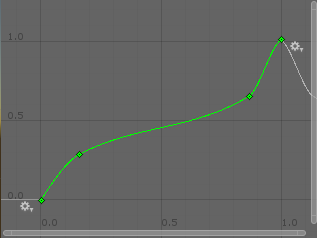
\includegraphics[width=.5\textwidth]{images/BoomerangAnimationCurve}
  \caption[The animation curve representing the change in \textbf{\textit{t}}]{This curve shows the change in \textbf{\textit{t}} as time goes from 0 to 1 on the x axis using Unity's AnimationCurve type.}
  \label{fig:boomerangcurve0}
\end{figure}

\begin{figure}[tbph]
    \centering
    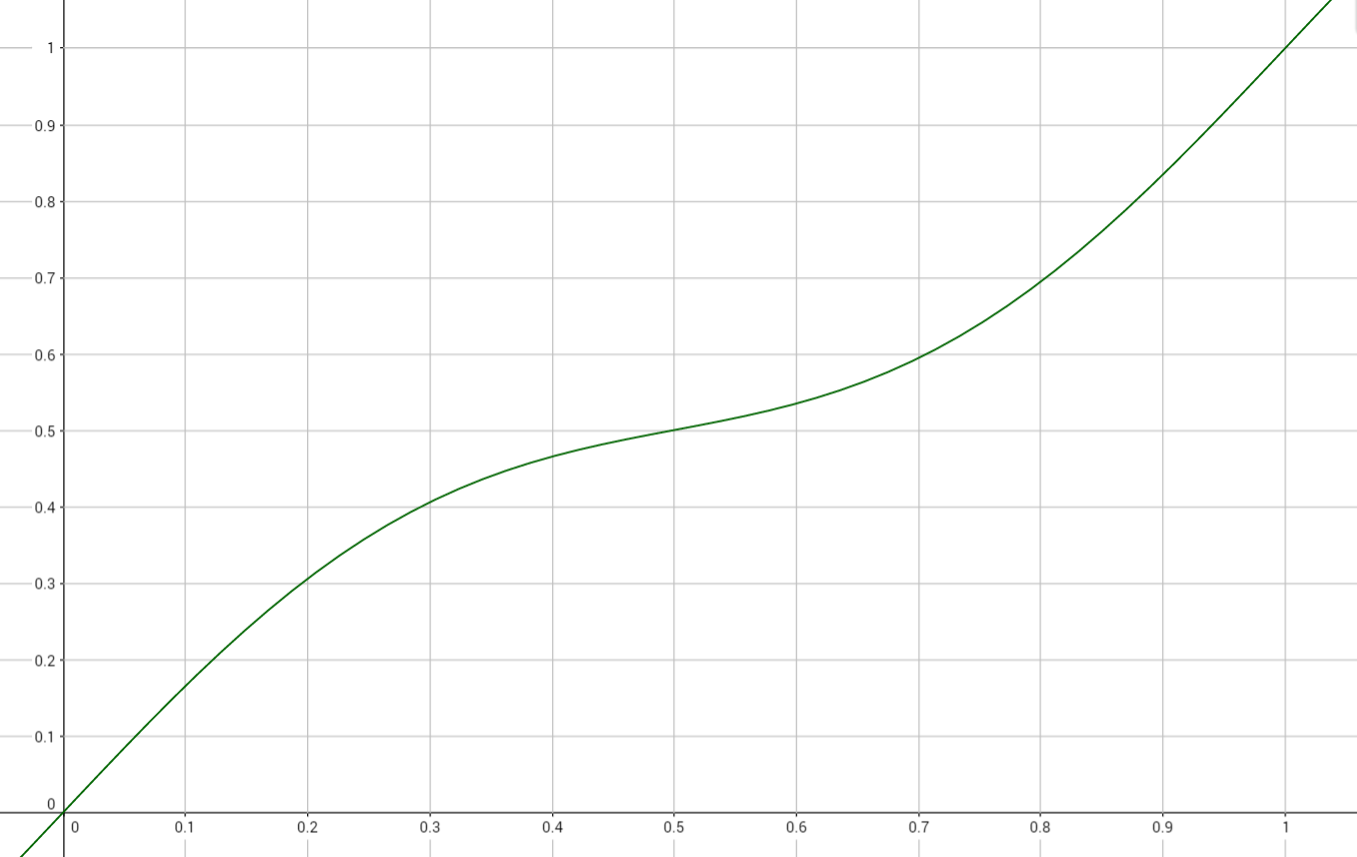
\includegraphics[width=.5\textwidth]{images/BoomerangMathematicalCurve}
    \caption[The mathematical curve representing the change in \textbf{\textit{t}}]{This curve shows the change in \textbf{\textit{t}} as time goes from 0 to 1 on the x axis using the mathematical curve $f(x) = x + sin(6.28x) / 9$}
    \label{fig:boomerangcurve1}
\end{figure}
    

As seen in Figure~\ref{fig:boomerangcurve0}, the AnimationCurve approach provides an easy to use interface with control points and control point handles, but there is also another way of solving the problem. 

A more generic approach would be to use a mathematical function like $f(x) = x + sin(x) / c$ to create a similar looking curve, but this approach has some problems that need to be dealt with. First of all, the curve needs to be scaled so that the wanted part of it is within the range of [0, 1] for both axes in order for the output to work with the interpolation function. This could be achieved by playing around with a graph plotting tool like GeoGebra or similar. In our case, the function $f(x) = x + sin(6.28x) / 9$ as seen in Figure~\ref{fig:boomerangcurve1} would provide similar behaviour to Figure~\ref{fig:boomerangcurve0}, but still lack the strong acceleration towards the end of the interpolation. This approach gives less control to the developers who work in the engine and spending time trying to scale the curves can be quite time consuming.

We also made sure to check the performance difference between the two approaches by measuring the execution time of both. We measured the time spent on each function per update and averaged out the time values after 10 boomerang throws. This gave us the following results:

\begin{itemize}
    \item The average execution time of the AnimationCurve's evaluation function took \textasciitilde$ 0.36 \mu s$
    \item The average execution time of the math function took \textasciitilde$ 0.20 \mu s$.
\end{itemize}

The time difference was calculated using Unity's Time.realTimeSinceStartup variable. The Time.realTimeSinceStartup float is measured in seconds so we multiplied the average time difference by $10^6$ and used a output precision of two decimals for these results. 
The mathematical approach provides a small increase in performance as seen from the results, but in our case the difference is too small to warrant using it. The AnimationCurve approach is far easier to work with directly in the editor instead of using external graph tools to modify the curve to our needs. On the contrary, the mathematical approach is more generic and might see use in non Unity applications.